\documentclass[letterpaper,11pt,twoside]{article}
\usepackage[utf8]{inputenc}
\usepackage{amsmath,amsfonts,amssymb,amsthm,latexsym}
\usepackage[spanish,es-noshorthands]{babel}
\usepackage[T1]{fontenc}
\usepackage{lmodern}
\usepackage{graphicx,hyperref}
\usepackage{tikz,pgf}
\usepackage{multicol}
\usepackage{fancyhdr}
\usepackage[height=9.5in,width=7in]{geometry}
\usepackage{fancyhdr}
\pagestyle{fancy}
\fancyhead[LE]{
\includegraphics[height=12pt]{Images/logo-colegio.png} Geometría $6^{\circ}$}
\fancyhead[RE]{}
\fancyhead[RO]{\textit{Germ\'an Avenda\~no Ram\'irez, Lic. U.D., M.Sc. U.N.}}
\fancyhead[LO]{}

\author{Germ\'an Avenda\~no Ram\'irez, Lic. U.D., M.Sc. U.N.}
\title{\begin{minipage}{.2\textwidth}

\includegraphics[height=1.75cm]{Images/logo-colegio.png}\end{minipage}
\begin{minipage}{.55\textwidth}
\begin{center}
Taller 04, Elementos gráficos\\
Geometría $6^{\circ}$
\end{center}
\end{minipage}\hfill
\begin{minipage}{.2\textwidth}

\includegraphics[height=1.75cm]{Images/logo-sed.png} 
\end{minipage}}
\date{}
\thispagestyle{plain}
\begin{document}
\maketitle
Nombre: \hrulefill Curso: \underline{\hspace*{44pt}} Fecha: \underline{\hspace*{2.5cm}}
\begin{multicols}{2}
 \section*{Lo que s\'e}
 Si realizaramos un mapa detallado de cada uno de los lugares por
los que nos movemos diarimente mientras realizamos nuestras
tareas diarias, el resultado sería un sin número de segmentos
unidos que podrían definir figuras y vértices.
\begin{itemize}
\item Lee la siguiente situación:
\end{itemize}
Guillermo quiere realizar un plano del recorrido que tiene
que hacer todos los días, para cumplir con sus tareas diarias.
\begin{enumerate}
\item[a.] Primera tarea: ordeñar las vacas y sacarlas a pastear.
\item[b.] Segunda tarea: recoger los huevos y darles de comer a las gallinas.
\item[c.] Tercera tarea: alimentar a los cerdos.
\item[d.] Cuarta tarea: llevar a las vacas de nuevo al corral.
\end{enumerate}
\begin{itemize}
\item Observa y copia la ubicación de los puntos que se muestran a
continuación. Piensa en el recorrido que hace Guillermo y traza
los caminos correspondientes.
\end{itemize}
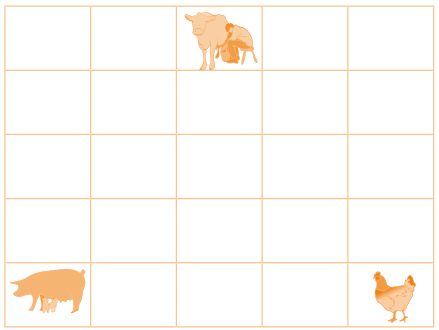
\includegraphics[scale=.55]{Images/animales_domesticos.png}
\begin{itemize}
\item ¿Qué figura se forma al trazar los recorridos?
\item Dibuja en tu cuaderno otra figura similar y explica
cuáles son las características comunes que tienen
entre sí.
\item Observa estas figuras y escribe en tu cuaderno qué las
diferencia de la que se obtuvo al dibujar el recorrido
hecho por Guillermo.
\end{itemize}
\begin{center}
\begin{tikzpicture}[scale=.85]
\filldraw[gray] (0,0)rectangle (3,2);
\filldraw[gray] (3.3,0)--(6.3,0)--(6.3,2) --cycle;
\filldraw[gray] (7.6,1) circle (1cm);
\end{tikzpicture}
\end{center}
\begin{itemize}
\item ¿Qué tipo de figura se formaría si antes de regresar las
vacas al corral, tuviera que ir a un sitio más? ¿Y a dos
sitios más? Realiza un dibujo que explique la situación
planteada.
\item Piensa en las actividades que realizas todos los días.
Recuerda la ubicación de los lugares en donde las haces
y representa los recorridos en un dibujo. ¿Qué figura
obtuviste?
\end{itemize}
\section*{Aprendo algo nuevo}
\begin{itemize}
\item Comencemos entonces, por diferenciar las figuras
abiertas y las cerradas.
\end{itemize}
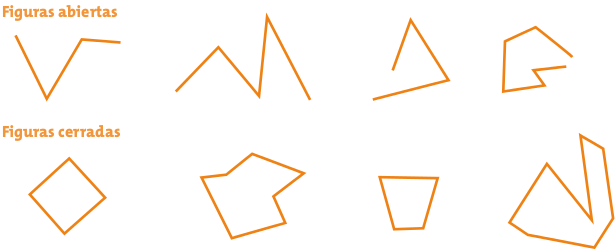
\includegraphics[scale=.8]{Images/Fig_abiertas_cerradas.png} 
\end{multicols}
\end{document}
